\documentclass[14pt]{article}
\usepackage[utf8]{inputenc}
\usepackage[T2A]{fontenc}
\usepackage[english]{babel} % Оставляем английский для поддержки, либо можно попробовать polyglossia для узбекской латиницы, но стандартно используют английский
\usepackage{amsmath, amssymb}
\usepackage{geometry}
\usepackage{graphicx}
\usepackage{xcolor}
\usepackage{hyperref}
\usepackage{tasks}
\usepackage{tcolorbox}
\tcbuselibrary{skins, breakable}
\usepackage{fancyhdr}
\usepackage{lastpage}
\usepackage{enumitem}

% Настройка геометрии
\geometry{a4paper, left=20mm, right=15mm, top=25mm, bottom=25mm, headheight=20pt}

% Цвета
\definecolor{taskblue}{RGB}{0, 102, 204}
\definecolor{lightorange}{RGB}{255, 240, 220}
\pagecolor{lightorange!10}

% Новый tcolorbox для задач (переведен заголовок)
\newtcolorbox[auto counter]{taskbox}[1][]{
  colback=white,
  colframe=taskblue,
  arc=5pt,
  boxrule=1.5pt,
  left=8pt,
  right=8pt,
  top=8pt,
  bottom=8pt,
  fonttitle=\bfseries\large,
  title=Savol \thetcbcounter, % <--- ПЕРЕВЕДЕНО
  breakable,
  pad at break=2mm,
  #1
}
% Настройка tasks (варианты ответов в две колонки)
\settasks{
  label=\Alph*),
  label-width=1.8em,
  item-indent=2.5em,
  column-sep=2em,
  before-skip=3pt,
  after-skip=3pt
}

% Колонтитулы (переведены или оставлены как есть, если это имена/названия)
\pagestyle{fancy}
\fancyhf{}
\fancyhead[L]{\textbf{MathCore} | MOCK Test-3}
\fancyhead[R]{Abdunazarov M.X.}
\fancyfoot[L]{\href{https://t.me/Math_Core_Dtm_MS_Att}{\textbf{MathCore}}}
\fancyfoot[R]{\href{https://t.me/Abd_mardon}{\textbf{@Abd\_mardon}}}
\fancyfoot[C]{\thepage/\pageref{LastPage}}
\renewcommand{\headrulewidth}{0.4pt}
\renewcommand{\footrulewidth}{0.4pt}

% Титульная страница (переведена)
\title{\Huge \textbf{MOCK Test-3}} % Название теста обычно не переводят
\author{Abdunazarov M.X.}
\date{}

\begin{document}

\maketitle

\begin{center}
    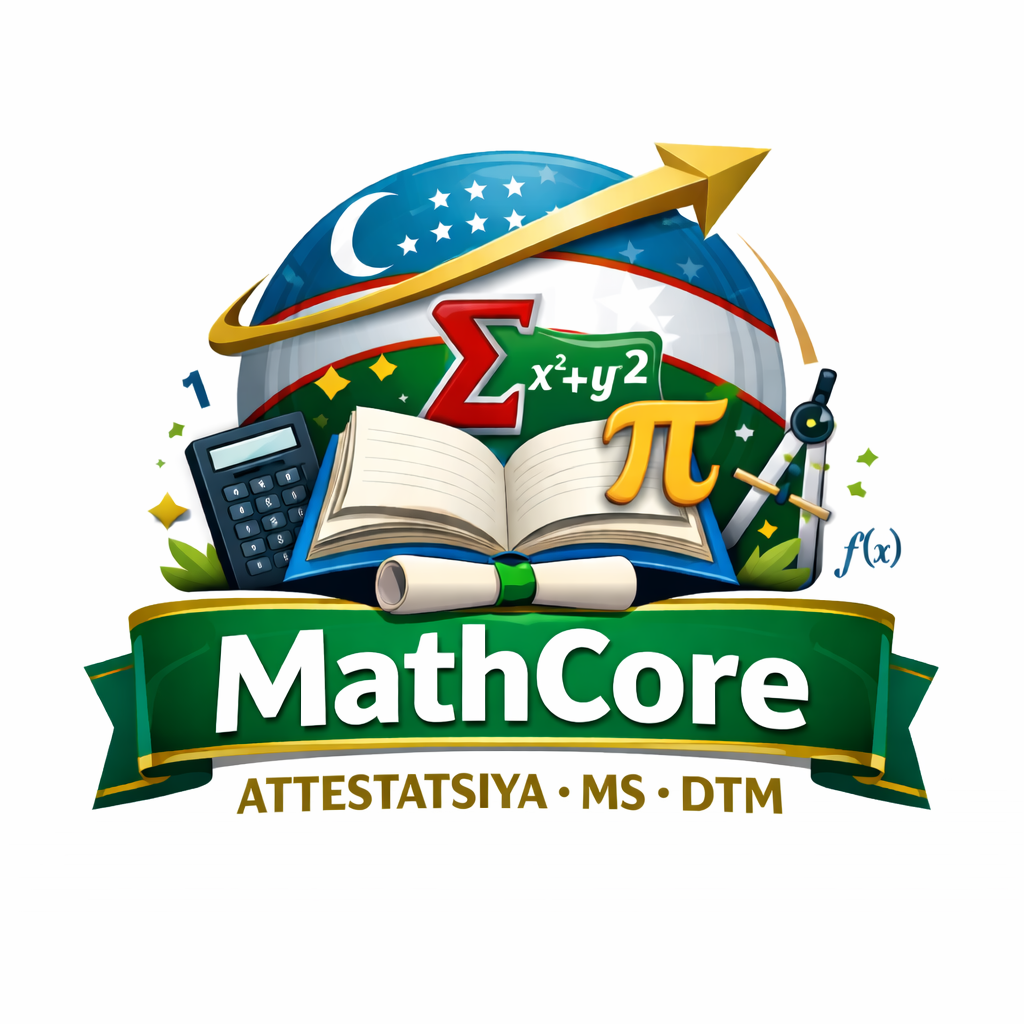
\includegraphics[width=0.3\textwidth]{logo.png} % Файл logo.png должен быть в папке с проектом
\end{center}
\vspace{1cm}

% --- Задача 1 ---
\begin{taskbox}
\(a\) ning qanday qiymatida \(y = x^2 - 2(a+1)x + 1\) parabolaning uchi \(y = \frac{3}{4}\) to'g'ri chiziqdan pastda joylashgan?
 \vspace{0.2cm} \begin{tasks}(2)
\task \((-\infty; -1) \cup (1; +\infty)\)
\task \((-\frac{1}{2}; \frac{3}{2})\)
\task \((-\infty; -\frac{3}{2}) \cup (-\frac{1}{2}; +\infty)\)
\task \((-\infty; -\frac{1}{2}) \cup (\frac{3}{2}; +\infty)\)
\end{tasks}
\vspace{2cm}
\end{taskbox}

% --- Задача 2 ---
\begin{taskbox}
210 sonining tub bo'lmagan natural bo'luvchilari soni nechta?
 \vspace{0.2cm} \begin{tasks}(2)
\task 16
\task 15
\task 12
\task 11
\end{tasks}
\vspace{2cm}
\end{taskbox}

% --- Задача 3 ---
\begin{taskbox}
\(a\) ning qanday qiymatlarida \(y = ax^2 - x + a\) parabolaning uchi \(Ox\) o'qidan yuqorida joylashgan?
 \vspace{0.2cm} \begin{tasks}(2)
\task \((-1; 0) \cup (1; +\infty)\)
\task \((-\frac{1}{2}; 0) \cup (\frac{1}{2}; +\infty)\)
\task \((-\infty; -\frac{1}{2}) \cup (\frac{1}{2}; +\infty)\)
\task \((-\frac{1}{2}; 0)\)
\end{tasks}
\vspace{2cm}
\end{taskbox}

% --- Задача 4 ---
\begin{taskbox}
Ma'lumki, \(\sin x = \frac{1}{3}\). \(\dfrac{\sin 2x - \sin 3x + \sin 5x}{1 + \cos x - 2\sin^2 2x}\) ifodaning qiymatini toping.
 \vspace{0.2cm} \begin{tasks}(2)
\task \(\frac{1}{2}\)
\task \(\frac{2}{5}\)
\task \(\frac{2}{3}\)
\task \(1\)
\end{tasks}
\vspace{2cm}
\end{taskbox}

% --- Задача 5 ---
\begin{taskbox}
\(\arccos(3x - 4) < \arccos(x - 2)\) tengsizlikni yeching.
 \vspace{0.2cm} \begin{tasks}(2)
\task \((1; +\infty)\)
\task \((-1; 5/3]\)
\task \([-1; 5/3]\)
\task \((1; 5/3]\)
\end{tasks}
\vspace{2cm}
\end{taskbox}

% --- Задача 6 ---
\begin{taskbox}
\(a\) parametrining qanday qiymatlarida \(\begin{cases} 3x + ay - 13 = 0 \\ 2x - 3y + 5 = 0 \end{cases}\) tenglamalar sistemasi yagona yechimga ega?
 \vspace{0.2cm} \begin{tasks}(2)
\task \(a \neq -4.5\)
\task \(a = -4.5\)
\task \(a = -6\)
\task \(a \neq -6\)
\end{tasks}
\vspace{2cm}
\end{taskbox}

% --- Задача 7 ---
\begin{taskbox}
10 dan kichik bo'lgan natural sonlardan nechtasi 10 bilan o'zaro tub?
 \vspace{0.2cm} \begin{tasks}(2)
\task 1
\task 2
\task 3
\task 4
\end{tasks}
\vspace{2cm}
\end{taskbox}

% --- Задача 8 ---
\begin{taskbox}
\(y = -3^x + 5\) funksiyasiga \((2,7)\) nuqtaga nisbatan simmetrik bo'lgan funksiyani toping.
 \vspace{0.2cm} \begin{tasks}(2)
\task \(y = 3^{x-4} + 9\)
\task \(y = 3^{-x+4} + 9\)
\task \(y = 3^{-x} - 5\)
\task \(y = 3^{x} - 5\)
\end{tasks}
\vspace{2cm}
\end{taskbox}

% --- Задача 9 ---
\begin{taskbox}
Arifmetik progressiyada \(S_8 = 32\) va \(S_{10} = 20\). \(S_{18}\) ni toping.
 \vspace{0.2cm} \begin{tasks}(2)
\task \(-120\)
\task \(-115\)
\task \(-110\)
\task \(-108\)
\end{tasks}
\vspace{2cm}
\end{taskbox}

% --- Задача 10 ---
\begin{taskbox}
Teng yonli trapetsiyaning asoslari 22 va 42 ga, yon tomonlari esa 26 ga teng. Uning yuzini toping.
 \vspace{0.2cm} \begin{tasks}(2)
\task 748
\task 768
\task 788
\task 808
\end{tasks}
\vspace{2cm}
\end{taskbox}

% --- Задача 11 ---
\begin{taskbox}
Konusning yon sirti to'la sirtining 60\% ini tashkil qiladi. Konus balandligining asos radiusiga nisbatini toping.
 \vspace{0.2cm} \begin{tasks}(2)
\task \(1.5\)
\task \(\frac{\sqrt{3}}{2}\)
\task \(\frac{\sqrt{5}}{2}\)
\task \(\frac{2}{3}\)
\end{tasks}
\vspace{2cm}
\end{taskbox}

% --- Задача 12 ---
\begin{taskbox}
ABCD trapetsiyasining AB va CD yon tomonlarida E va F nuqtalari shunday olinganki, AF va ED kesmalari O nuqtada kesishadi. Ma'lumki, \(BC:AD = 1:2\), \(AE:AB = 1:2\), \(FD:CD = 2:3\) va trapetsiyaning yuzi 30 ga teng. AOE uchburchak yuzini toping.
\begin{center}

\includegraphics[width=0.4\textwidth]{1.png} % Файл 1.png должен быть в папке с проектом
\end{center}
 \vspace{0.2cm} \begin{tasks}(2)
\task 10
\task \(\frac{5}{2}\)
\task \(\frac{20}{3}\)
\task \(\frac{10}{3}\)
\end{tasks}
\vspace{2cm}
\end{taskbox}

% --- Задача 13 ---
\begin{taskbox}
Rasmda tasvirlangan teng yonli ABCD trapetsiyasi uchun \(CE:ED = 2:3\), \(BC = 8\), \(AD = 12\) ekanligi ma'lum. \(S_{ABE}:S_{ADE}\) nisbatni toping.
\begin{center}

\includegraphics[width=0.4\textwidth]{2.png} % Файл 2.png должен быть в папке с проектом
\end{center}
 \vspace{0.2cm} \begin{tasks}(2)
\task 5:4
\task 6:5
\task 4:3
\task 3:2
\end{tasks}
\vspace{2cm}
\end{taskbox}

% --- Задача 14 ---
\begin{taskbox}
Birinchi idishda 5 ta yaroqli va 5 ta yaroqsiz detal, ikkinchisida – 7 ta yaroqli va 3 ta yaroqsiz, uchinchisida – 8 ta yaroqli va 2 ta yaroqsiz detal bor. Tavakkaliga olingan detalning yaroqli chiqishi va u birinchi idishdan olingan bo'lish ehtimolini toping.
 \vspace{0.2cm} \begin{tasks}(2)
\task 0.21
\task 0.23
\task 0.2
\task 0.25
\end{tasks}
\vspace{2cm}
\end{taskbox}

% --- Задача 15 ---
\begin{taskbox}
Katta aka uydan maktabgacha masofani 24 daqiqada, kichik aka esa 30 daqiqada bosib o'tadi. Agar katta aka uydan kichik akadan 3 daqiqa keyin chiqsa, u kichik akani necha daqiqada quvib yetadi?
 \vspace{0.2cm} \begin{tasks}(2)
\task 12
\task 15
\task 18
\task 24
\end{tasks}
\vspace{2cm}
\end{taskbox}

% --- Задача 16 ---
\begin{taskbox}
ABC uchburchakning AB tomonida D nuqtasi olingan: \(AD = 4\), \(DB = 5\), \(BC = 12\), \(AC = 6\). CD kesma uzunligini toping.
\begin{center}

\includegraphics[width=0.4\textwidth]{3.png} % Файл 3.png должен быть в папке с проектом
\end{center}
 \vspace{0.2cm} \begin{tasks}(2)
\task 6
\task 8
\task 7
\task 9
\end{tasks}
\vspace{2cm}
\end{taskbox}

% --- Задача 17 ---
\begin{taskbox}
\([0; \pi]\) kesmada \(\sin^2 x < \cos^2 x - \frac{\sqrt{3}}{2}\) tengsizlikni yeching.
 \vspace{0.2cm} \begin{tasks}(2)
\task \(x \in [0; \frac{\pi}{12}) \cup (\frac{11\pi}{12}; \pi]\)
\task \(x \in [\frac{\pi}{12}; \frac{11\pi}{12}]\)
\task \(x \in [0; \frac{5\pi}{12})\)
\task \(x \in [0; \pi]\)
\end{tasks}
\vspace{2cm}
\end{taskbox}

% --- Задача 18 ---
\begin{taskbox}
Uchta idish bor. Birinchisida 5 ta ko'k va 3 ta qizil shar, ikkinchisida 4 ta ko'k va 4 ta qizil, uchinchisida 5 ta qizil va 3 ta ko'k shar bor. Tavakkaliga idish tanlanadi va undan bitta shar olinadi. Sharning qizil bo'lish ehtimolini toping.
 \vspace{0.2cm} \begin{tasks}(2)
\task \(\frac{1}{4}\)
\task \(\frac{1}{3}\)
\task \(\frac{1}{2}\)
\task \(\frac{3}{4}\)
\end{tasks}
\vspace{2cm}
\end{taskbox}

% --- Задача 19 ---
\begin{taskbox}
\(27^3 + 37^3\) yig'indisining 13 ga bo'lgandagi qoldiqni toping.
 \vspace{0.2cm} \begin{tasks}(2)
\task 6
\task 3
\task 5
\task 7
\end{tasks}
\vspace{2cm}
\end{taskbox}

% --- Задача 20 ---
\begin{taskbox}
\((x + y)^n\) yoyilmasining koeffitsiyentlari yig'indisi 4096 ga teng. Ko'phadning eng katta koeffitsiyentini toping.
 \vspace{0.2cm} \begin{tasks}(2)
\task 792
\task 864
\task 924
\task 936
\end{tasks}
\vspace{2cm}
\end{taskbox}

% --- Задача 21 ---
\begin{taskbox}
Rasmda berilgan ma'lumotlarga asosan BDC uchburchak yuzini toping.
\begin{center}

\includegraphics[width=0.4\textwidth]{4.png} % Файл 4.png должен быть в папке с проектом
\end{center}
 \vspace{0.2cm} \begin{tasks}(2)
\task \(18\sqrt{3}\)
\task \(16\sqrt{3}\)
\task \(15\sqrt{3}\)
\task \(24\sqrt{3}\)
\end{tasks}
\vspace{2cm}
\end{taskbox}

% --- Задача 22 ---
\begin{taskbox}
\(\sqrt{-x^2 + 6x - 4} > x - 4\) tengsizlikni qancha butun son qanoatlantiradi?
 \vspace{0.2cm} \begin{tasks}(2)
\task 1
\task 2
\task 3
\task 4
\end{tasks}
\vspace{2cm}
\end{taskbox}

% --- Задача 23 ---
\begin{taskbox}
\(\sin 20^\circ \cdot \sin 40^\circ \cdot \sin 80^\circ\) ni hisoblang.
 \vspace{0.2cm} \begin{tasks}(2)
\task \(\frac{\sqrt{3}}{4}\)
\task \(\frac{\sqrt{3}}{8}\)
\task \(\frac{\sqrt{3}}{16}\)
\task \(\frac{\sqrt{3}}{2}\)
\end{tasks}
\vspace{2cm}
\end{taskbox}

% --- Задача 24 ---
\begin{taskbox}
\(y = -x^2 + 2x\) funksiya grafigini \(Ox\) o'qi atrofida aylantirishdan hosil bo'lgan jism hajmini toping.
 \vspace{0.2cm} \begin{tasks}(2)
\task \(\frac{15\pi}{14}\)
\task \(\frac{17\pi}{16}\)
\task \(\frac{16\pi}{15}\)
\task \(\frac{13\pi}{12}\)
\end{tasks}
\vspace{2cm}
\end{taskbox}

% --- Задача 25 ---
\begin{taskbox}
4 xil turdagi ruchkalar mavjud bo'lsa, 7 ta ruchkani necha xil usulda tanlash mumkin? (Har bir turdagi ruchkalar bir-biridan farqsiz deb hisoblanadi.)
 \vspace{0.2cm} \begin{tasks}(2)
\task 120
\task 56
\task 16384
\task 2401
\end{tasks}
\vspace{2cm}
\end{taskbox}

% --- Задача 26 ---
\begin{taskbox}
Funksiyaning ekstrimumlarini toping:
\[
y = x^3 - 6x^2 + 9x + 5
\]
 \vspace{0.2cm} \begin{tasks}(2)
 \task Minimum:  $x = 1$, maksimum: $x = 3$
\task Minimum:  $x = 3$, maksimum: $x = 1$
\task Minimum:  $x = 0$, maksimum: $x = 2$
\task Ekstrimumlar yo'q
 
\end{tasks}
\vspace{2cm}
\end{taskbox}

% --- Задача 27 ---
\begin{taskbox}
\([0; \pi]\) kesmada \(\sin 3x \cdot \cos 2x - \cos 3x \cdot \sin 2x = \frac{1}{2}\) tenglama ildizlari yig'indisini toping.
 \vspace{0.2cm} \begin{tasks}(2)
\task \(\pi\)
\task \(\frac{3\pi}{2}\)
\task \(\frac{2\pi}{3}\)
\task ildizlari yo'q
\end{tasks}
\vspace{2cm}
\end{taskbox}

% --- Задача 28 ---
\begin{taskbox}
Agar \(g(x) = x^3 f(x)\) kamayuvchi funksiya bo'lsa, quyidagi tengsizliklardan qaysi biri doimo o'rinli?
 \vspace{0.2cm} \begin{tasks}(2)
\task \(f(x) > f'(x)\)
\task \(x f'(x) < -3f(x)\)
\task \(f'(x) > f(x)\)
\task \(x^2 f(x) > x f'(x)\)
\end{tasks}
\vspace{2cm}
\end{taskbox}

% --- Задача 29 ---
\begin{taskbox}
Rasmda \(y = 2x^2\) va \(y = 4 - x\) funksiyalarining grafiklari tasvirlangan. Ular orasidagi sohaga ichki chizilgan to'g'ri to'rtburchak yuzining maksimal qiymatini toping.
\begin{center}

\includegraphics[width=0.4\textwidth]{6.png} % Файл 6.png должен быть в папке с проектом
\end{center}
 \vspace{0.2cm} \begin{tasks}(2)
\task \(\frac{35}{22}\)
\task \(\frac{44}{27}\)
\task \(\frac{47}{26}\)
\task \(\frac{49}{35}\)
\end{tasks}
\vspace{2cm}
\end{taskbox}

% --- Задача 30 ---
\begin{taskbox}
Maktab oshxonasida 4 xil shirinlik bor. O'quvchi 5 ta shirinlikni necha xil usulda tanlashi mumkin? (Tartib muhim emas, bir turdagi shirinliklar farqsiz.)
 \vspace{0.2cm} \begin{tasks}(2)
\task 1024
\task 625
\task 56
\task 120
\end{tasks}
\vspace{2cm}
\end{taskbox}

% --- Задача 31 ---


\begin{taskbox}
Teng;amaning barcha yechimlarini toping:
\[
2\sin^2 x - 3\sin x + 1 = 0, \quad x \in [0, 2\pi].
\]

 \vspace{0.2cm} \begin{tasks}(2)
\task  $x = \frac{\pi}{6}, \frac{5\pi}{6}$
\task $x = \frac{\pi}{4}, \frac{3\pi}{4}$
\task $x = \frac{\pi}{3}, \frac{2\pi}{3}$
\task $x = 0, \pi$
\end{tasks}
\vspace{2cm}
\end{taskbox}
% --- Задача 32 ---
\begin{taskbox}
ABCD to'g'ri to'rtburchakdan ECD uchburchak kesib olingan. \(AB = 6\), \(AD = ED\). Yuzi maksimal bo'lganda, ABED to'rtburchak yuzini toping.
\begin{center}

\includegraphics[width=0.4\textwidth]{8.png} % Файл 8.png должен быть в папке с проектом
\end{center}
 \vspace{0.2cm} \begin{tasks}(2)
\task \(18\sqrt{3}\)
\task \(16\sqrt{3}\)
\task \(14\sqrt{3}\)
\task \(12\sqrt{3}\)
\end{tasks}
\vspace{2cm}
\end{taskbox}

% --- Задача 33 ---
\begin{taskbox}
Agar \(a \parallel b\) bo'lsa, \(\alpha\) burchakni toping.
\begin{center}

\includegraphics[width=0.4\textwidth]{9.png} % Файл 9.png должен быть в папке с проектом
\end{center}
 \vspace{0.2cm} \begin{tasks}(2)
\task \(140^\circ\)
\task \(160^\circ\)
\task \(150^\circ\)
\task \(120^\circ\)
\end{tasks}
\vspace{2cm}
\end{taskbox}

% --- Задача 34 ---
\begin{taskbox}
To'g'ri burchakli uchburchakka ichki chizilgan aylana radiusini toping.
\begin{center}
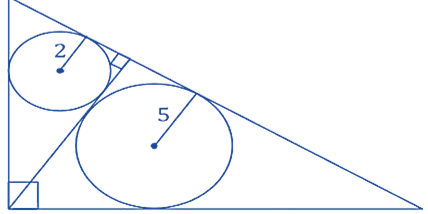
\includegraphics[width=0.4\textwidth]{10.png} % Файл 10.png должен быть в папке с проектом
\end{center}
 \vspace{0.2cm} \begin{tasks}(2)
\task 3
\task 7
\task \(\sqrt{29}\)
\task \(\sqrt{21}\)
\end{tasks}
\vspace{2cm}
\end{taskbox}

% --- Задача 35 --- (Исправлена, так как в оригинале текст обрывался)
\begin{taskbox}
\(A\) va \(B\) shaharlari orasidagi masofa 120 km. Poyezd yo'lning o'rtasida 10 daqiqa to'xtadi va harakatni dastlabki tezligidan 12 km/soat ko'proq tezlikda davom ettirdi. Agar butun yo'l uchun 2 soat 25 minut ketgan bo'lsa poyezdning dastlabki tezligini toping.

\vspace{0.2cm} \begin{tasks}(2) % 
\task 45
\task 52
\task 44
\task 48
\end{tasks}
\vspace{2cm}
\end{taskbox}
% ПРИМЕЧАНИЕ: Для задачи 35 в оригинале не было вариантов ответа, я поставил заглушку. Вам нужно их добавить.

\end{document}